% =====================================================================
\chapter{Arbitrage statistique multi-actifs}
\label{ch:10}
% =====================================================================

\section{Objectifs et organisation du chapitre}

\paragraph{Objectifs.} Une paire est un cas particulier : on couvre une action par une autre. Plus généralement, on peut couvrir chaque action par les facteurs communs à tout le marché et trader ce qui reste, son \emph{résidu}. C'est l'approche d'\citet{avellaneda2010}, qui a structuré l'arbitrage statistique institutionnel sur actions. À la fin du chapitre, vous saurez : (1) dériver l'analyse en composantes principales (ACP) et construire des portefeuilles propres ; (2) distinguer les vrais facteurs du bruit d'estimation (borne de Marchenko-Pastur) ; (3) modéliser les résidus par un processus d'Ornstein-Uhlenbeck et calculer le \emph{s-score} ; (4) implémenter et tester la stratégie complète ; (5) situer les approches de portefeuilles de retour à la moyenne parcimonieux.

\paragraph{Code.} \texttt{code/ch10/ch10\_pca\_statarb.py}.

% =====================================================================
\section{L'analyse en composantes principales}
% =====================================================================

\subsection{Le problème}

Soit $C$ la matrice de corrélation des rendements standardisés de $N$ actions ($N\times N$, symétrique, positive). On cherche la combinaison $w$ (de norme 1) dont la variance $w^\top Cw$ est maximale : la direction qui explique le plus de mouvements communs.

\begin{proposition}\label{c10:prop:pca}
Le maximum de $w^\top Cw$ sous la contrainte $w^\top w = 1$ est atteint en $w = v_1$, vecteur propre associé à la plus grande valeur propre $\lambda_1$ de $C$, et vaut $\lambda_1$. Les composantes suivantes sont les vecteurs propres suivants, orthogonaux entre eux.
\end{proposition}
\begin{proof}
On introduit un multiplicateur de Lagrange $\lambda$ et l'on annule le gradient de $w^\top Cw - \lambda(w^\top w - 1)$ : $2Cw - 2\lambda w = 0$, soit $Cw = \lambda w$. Les candidats sont donc les vecteurs propres de $C$, et pour un tel vecteur la variance vaut $w^\top Cw = \lambda w^\top w = \lambda$. Le maximum est atteint pour la plus grande valeur propre. Pour la deuxième composante, on ajoute la contrainte d'orthogonalité à $v_1$ et le même raisonnement donne $v_2$.
\end{proof}

La somme des valeurs propres vaut $\mathrm{tr}(C) = N$ ; la part de variance expliquée par les $k$ premières composantes est $\sum_{j\le k}\lambda_j/N$. Sur les actions, la première composante est presque toujours le \og marché\fg{} (tous les poids de même signe), les suivantes opposent des secteurs ou des styles.

\paragraph{Portefeuilles propres.} Les vecteurs propres portent sur des rendements standardisés ; pour obtenir un portefeuille investissable, on divise chaque poids par la volatilité de l'action : $Q_{ij} = v_{j,i}/\sigma_i$. Le rendement du facteur $j$ est $F_{jt} = \sum_iQ_{ij}R_{it}$.

\subsection{Combien de facteurs ? La borne de Marchenko-Pastur}

Même si les actions étaient indépendantes, la matrice de corrélation estimée sur $T$ jours aurait des valeurs propres dispersées autour de 1, par pur bruit d'échantillonnage. La théorie des matrices aléatoires montre que, pour des séries indépendantes et $N/T = q$ fixé, les valeurs propres se répartissent entre $(1-\sqrt q)^2$ et $(1+\sqrt q)^2$. Une valeur propre au-dessus de $(1+\sqrt q)^2$ signale un facteur réel ; celles en dessous sont indiscernables du bruit.

\begin{codebox}[ — E1, spectre et borne de Marchenko-Pastur]
\textbf{Protocole :} 100 actions simulées avec 3 facteurs, fenêtre de 252 jours ($q = 0{,}40$, borne $2{,}66$). \textbf{Résultats :} valeurs propres $29{,}7$ ; $10{,}4$ ; $6{,}8$ ; puis $1{,}42$ ; $1{,}39$\dots{} Exactement trois valeurs propres dépassent la borne ; elles expliquent 47\,\% de la variance.
\end{codebox}

\begin{figure}[h]
\centering
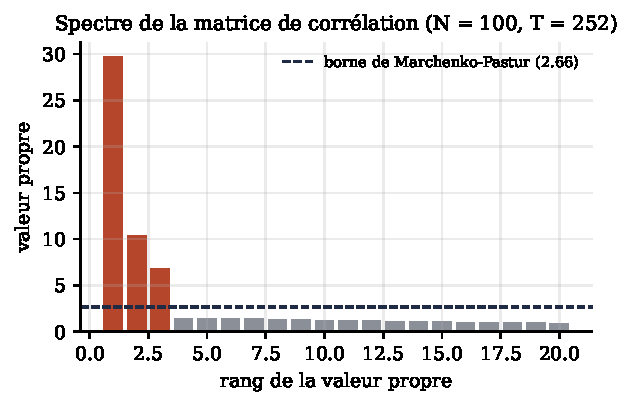
\includegraphics[width=0.62\textwidth]{ch10/spectre_valeurs_propres.pdf}
\caption{Les 20 plus grandes valeurs propres de la matrice de corrélation ; en rouge, celles qui dépassent la borne de Marchenko-Pastur.}
\label{c10:fig:spectrum}
\end{figure}

% =====================================================================
\section{Le modèle d'Avellaneda et Lee}
% =====================================================================

\subsection{Décomposition des rendements}

Chaque action suit
\[
\frac{\dd P_{it}}{P_{it}} = \alpha_i\,\dd t + \sum_{j=1}^{k}\beta_{ij}\,F_{jt}\,\dd t + \dd X_{it},
\]
où les $F_j$ sont les rendements des facteurs (portefeuilles propres ou ETF sectoriels) et $X_{it}$ est le \emph{résidu cumulé}, supposé suivre un processus d'Ornstein-Uhlenbeck (chapitre~5) : $\dd X_{it} = \kappa_i(m_i - X_{it})\dd t + \sigma_i\dd W_{it}$. Une position longue sur l'action et courte sur $\beta_{ij}$ unités de chaque facteur n'est exposée qu'à $X_{it}$.

\begin{intuition}
Chaque action est un passager dans un bus (le marché) qui roule vite et change de direction. Le chauffeur, c'est le facteur ; on ne sait pas où il va. Mais chaque passager se déplace aussi dans l'allée, et il finit toujours par revenir à sa place. On ne parie pas sur la route du bus ; on parie que le passager qui est trop loin de sa place va y retourner.
\end{intuition}

\subsection{Estimation, pas à pas}

Chaque jour $t$ :
\begin{enumerate}
\item \textbf{Facteurs :} ACP sur la matrice de corrélation des 252 derniers jours ; on garde $k$ portefeuilles propres.
\item \textbf{Régression :} pour chaque action, régression de ses rendements des 60 derniers jours sur ceux des facteurs ; on obtient $\hat\beta_{ij}$ et les résidus $\hat\varepsilon_{is}$.
\item \textbf{Résidu cumulé :} $X_{is} = \sum_{u\le s}\hat\varepsilon_{iu}$ sur la fenêtre.
\item \textbf{AR(1) :} $X_{i,s+1} = a_i + b_iX_{is} + \zeta_{i,s+1}$ ; d'où, par la correspondance du chapitre~5, $\kappa_i = -252\ln b_i$, $m_i = a_i/(1-b_i)$ et $\sigma_{eq,i} = \sqrt{\Var(\zeta_i)/(1-b_i^2)}$.
\item \textbf{s-score :} $s_i = (X_{it} - m_i)/\sigma_{eq,i}$ : l'écart actuel du résidu à son équilibre, en écarts-types stationnaires.
\end{enumerate}

\subsection{Règles de trading}

Avellaneda et Lee utilisent des seuils asymétriques : ouvrir une position courte si $s_i > 1{,}25$ et longue si $s_i < -1{,}25$ ; fermer la position courte quand $s_i < 0{,}75$ et la longue quand $s_i > -0{,}5$. Ils ne tradent que les actions dont le retour est assez rapide : $\kappa_i > 252/30$, soit un temps caractéristique $1/\kappa_i$ inférieur à environ 30 jours de bourse, une demi-vie inférieure à une vingtaine de jours. Chaque position est couverte par les facteurs, de sorte que le portefeuille est proche de la neutralité au marché.

\paragraph{Résultats publiés.} Selon le résumé de l'article, la version ACP affiche un ratio de Sharpe annuel moyen de $1{,}44$ sur 1997–2007 sur les actions américaines, avec une performance plus forte avant 2003 ; l'ajout d'une information de volume améliore les résultats.

% =====================================================================
\section{Expérience}
% =====================================================================

\begin{codebox}[ — E2 et E3, stratégie s-score sur univers simulé]
\textbf{Protocole :} 100 actions, 3 facteurs, 1\,000 jours de trading. Scénario \og signal\fg{} : résidus cumulés OU de demi-vie 8 jours (écart-type stationnaire 3\,\%) plus un bruit quotidien ; scénario \og nul\fg{} : résidus en bruit blanc de même variance quotidienne. \textbf{Résultats} (rendement annuel ; ratio de Sharpe) :
\begin{center}\small
\begin{tabular}{lccc}
\toprule
 & 0 pb & 5 pb & 10 pb\\
\midrule
Signal, $k = 1$ facteur & $9{,}1\,\%$ ; 4,1 & $8{,}2\,\%$ ; 3,7 & $7{,}3\,\%$ ; 3,3\\
Signal, $k = 3$ facteurs & $10{,}5\,\%$ ; 9,0 & $9{,}6\,\%$ ; 8,2 & $8{,}6\,\%$ ; 7,4\\
Signal, $k = 10$ facteurs & $10{,}1\,\%$ ; 8,4 & $9{,}0\,\%$ ; 7,5 & $8{,}0\,\%$ ; 6,7\\
Nul, $k = 3$ & $-0{,}1\,\%$ ; $-0{,}1$ & $-1{,}0\,\%$ ; $-0{,}8$ & $-1{,}9\,\%$ ; $-1{,}4$\\
\bottomrule
\end{tabular}
\end{center}
\end{codebox}

\begin{figure}[h]
\centering
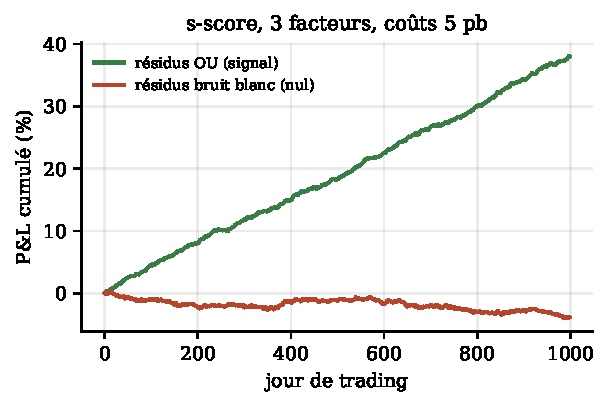
\includegraphics[width=0.62\textwidth]{ch10/pnl_sscore.pdf}
\caption{P\&L cumulé de la stratégie s-score (3 facteurs, 5 pb) quand les résidus reviennent à la moyenne et quand ils ne le font pas.}
\label{c10:fig:pnl}
\end{figure}

\paragraph{Lecture.} (1) Avec un seul facteur, une partie du risque sectoriel reste dans les résidus : la volatilité double et le Sharpe est divisé par deux. Avec trop de facteurs (10 au lieu de 3), on retire un peu de signal avec le bruit. Le bon nombre est celui que suggère Marchenko-Pastur. (2) Sans retour à la moyenne des résidus, la méthode ne gagne rien et perd ses coûts : elle ne crée pas d'avantage, elle l'exploite. (3) Les Sharpe de 8 du monde simulé sont irréalistes : le modèle y est exactement vrai, les paramètres constants, l'exécution parfaite. La valeur publiée de $1{,}44$, en déclin, donne l'ordre de grandeur réel.

\begin{pitfall}
Cette stratégie fait beaucoup de transactions sur beaucoup de titres : les coûts, l'impact et le coût d'emprunt des titres vendus à découvert y sont déterminants. Elle est aussi typiquement \og encombrée\fg : lors de la crise d'août 2007, de nombreux fonds détenant des portefeuilles semblables ont dû liquider en même temps \citep{khandanilo2011}. Pour un particulier, l'univers doit rester restreint aux titres très liquides et faciles à emprunter.
\end{pitfall}

% =====================================================================
\section{Portefeuilles de retour à la moyenne parcimonieux}
% =====================================================================

Plutôt que de couvrir chaque action par des facteurs, on peut chercher directement la combinaison d'actifs la plus prévisible. \citet{boxtiao1977} posent le problème pour un VAR(1) $x_t = Ax_{t-1} + \varepsilon_t$ : la prévisibilité d'un portefeuille $w$ est le rapport entre la variance de sa partie prévue et sa variance totale, $\lambda(w) = w^\top A\Gamma A^\top w/w^\top\Gamma w$ (avec $\Gamma$ la covariance de $x$). Minimiser $\lambda$ donne le portefeuille qui revient le plus vite à la moyenne ; c'est un problème de valeur propre généralisée, de même nature que la proposition~\ref{c10:prop:pca}. \citet{daspremont2011} ajoute une contrainte de parcimonie (peu d'actifs non nuls) pour obtenir des portefeuilles tradables à faibles coûts.

% =====================================================================
\section{Ce que la théorie apporte, et ses limites}
% =====================================================================

\paragraph{Apports.} Une généralisation naturelle du \emph{pairs trading} à tout un univers, une neutralisation explicite des risques communs, un critère objectif du nombre de facteurs, et un signal (le \emph{s-score}) directement issu du modèle OU.

\paragraph{Limites.} Facteurs instables d'une fenêtre à l'autre (les vecteurs propres peuvent changer de signe ou d'ordre) ; estimation sur 60 jours très bruitée ; coûts élevés ; profits historiques en déclin ; risque de foule. L'approche demande une infrastructure de données et d'exécution plus lourde que le \emph{pairs trading} simple.

% =====================================================================
\section{Fiche à recopier au tableau blanc}
% =====================================================================

\begin{whiteboard}
\begin{itemize}[leftmargin=1.2em]
\item \textbf{ACP :} $\max_w w^\top Cw$ s.c. $w^\top w=1$ $\Rightarrow$ $Cw = \lambda w$ ; part expliquée $\sum_{j\le k}\lambda_j/N$.
\item \textbf{Portefeuille propre :} $Q_{ij} = v_{j,i}/\sigma_i$, $F_{jt} = \sum_iQ_{ij}R_{it}$.
\item \textbf{Marchenko-Pastur :} bruit entre $(1\pm\sqrt{N/T})^2$.
\item \textbf{Modèle :} $R_i = \alpha_i + \sum_j\beta_{ij}F_j + \dd X_i$, $X_i$ OU.
\item \textbf{AR(1) sur $X$ :} $\kappa = -252\ln b$, $m = a/(1-b)$, $\sigma_{eq} = \sqrt{\Var(\zeta)/(1-b^2)}$.
\item \textbf{s-score :} $s = (X - m)/\sigma_{eq}$ ; ouvrir à $\pm1{,}25$, fermer court à $0{,}75$, long à $-0{,}5$ ; filtre $\kappa > 252/30$.
\item \textbf{Box-Tiao :} minimiser $w^\top A\Gamma A^\top w/w^\top\Gamma w$.
\end{itemize}
\end{whiteboard}

% =====================================================================
\section{Exercices}
% =====================================================================

\begin{exercise}
Montrez que deux vecteurs propres d'une matrice symétrique associés à des valeurs propres distinctes sont orthogonaux. Pourquoi les rendements des portefeuilles propres sont-ils alors non corrélés sur la fenêtre d'estimation ?
\end{exercise}

\begin{exercise}
Calculez la borne de Marchenko-Pastur pour 500 actions et 252 jours, puis pour 500 actions et 1\,000 jours. Commentez.
\end{exercise}

\begin{exercise}
Avec $b = 0{,}9$ sur données quotidiennes, calculez $\kappa$ et la demi-vie. Le titre passe-t-il le filtre d'Avellaneda et Lee ?
\end{exercise}

\begin{exercise}[à coder]
Remplacez les portefeuilles propres par un seul facteur \og marché\fg{} égal à la moyenne des rendements et comparez avec $k = 1$ en ACP.
\end{exercise}

\begin{exercise}[données réelles]
Construisez un univers de 30 à 50 ETF ou actions très liquides (via Interactive Brokers) et calculez le spectre de leur matrice de corrélation sur un an. Combien de valeurs propres dépassent la borne ?
\end{exercise}

% =====================================================================
\section{Pour aller plus loin}
% =====================================================================

\begin{toread}
\begin{itemize}[leftmargin=1.2em]
\item \citet{avellaneda2010} : la section sur la construction des facteurs (ACP et ETF), celle sur le \emph{s-score} et l'annexe sur l'estimation des paramètres OU.
\item \citet{boxtiao1977} et \citet{daspremont2011} : portefeuilles de retour à la moyenne.
\item \citet{khandanilo2011} : ce qui arrive quand tout le monde trade la même chose.
\item \citet{guijarro2021} : la version \og apprentissage profond\fg{} des signaux sur résidus, reprise au chapitre~11.
\end{itemize}
\end{toread}

\section{Scripts du chapitre}
\noindent\texttt{code/ch10/ch10\_pca\_statarb.py} : E1 (figure~\ref{c10:fig:spectrum}), E2–E3 (figure~\ref{c10:fig:pnl}).
